\chapter{Introduction au P/Invoke}

\section{Commençons}
Tout d'abord, créer un dossier 'ChapterTwo' pour le projet et créer un nouveau fichier, 'ChapTwo.c' dans le dossier 'ChapterTwo'.

Supposons que nous ayons une fonction d’addition de base dans une bibliothèque C que nous voulons appeler.

\lstinputlisting[style=customc, language=C]{codes/Chap2/Chap2Snippet1.c}

Au premier abord nous pourrions croire qu'il s'agit d'une simple opération d'addition, mais il y a quelques considérations qui doivent être observées d'abord avant d'essayer d'écrire le code d'enveloppe d'invocation de plate-forme pour la fonction ci-dessus :

\begin{enumerate}
	\item \label{itm:first} le type `int` en C peut être considéré comme long de 2 ou 4 octets ou aussi long qu'il puisse être selon l'architecture et le compilateur sur lequel la bibliothèque est compilée. Dans la norme C, int doit être capable de contenir \textbf{au moins} l'intervalle [\textminus32,767, +32,767]; ainsi, sa taille est d'au moins 16 bits.
	
	\item En raison de \ref{itm:first}, vous pouvez raisonnablement vous prémunir contre la perte de données en remplaçant C\# Int32(int) qui contient 4 octets, ou vous pouvez choisir de suivre la norme strictement en fournissant C\# Int16(short) qui contient 2 octets, même s'il peut subir des pertes de données. La meilleure approche est d'éviter d'utiliser "au moins" des entiers en C et d'utiliser des entiers de taille fixe fournis par le compilateur dans le fichier ''stdint.h'' si vous avez gardé à l'esprit l'interface de la fonction externe..
	
	\item Parfois, il faut garder à l'esprit l'endianité, bien qu'elle soit moins préoccupante dans les architecture x86\_64 la petite endianesse est la valeur par défaut.
\end{enumerate}
La meilleure approche pour écrire la fonction Addition est d'indiquer clairement la taille des entiers que vous essayez d'ajouter si possible.

\lstinputlisting[style=customc, language=C]{codes/Chap2/Chap2Snippet2.c}

\section{Compiler la Library}
Ce livre suppose que vous avez une connaissance suffisante de C, nous vous fournirons tout de même des instructions de compilation. La commande suivante suppose que vous avez nommé votre fichier de code source : ' ChapTwo.c' comme indiqué au début de ce chapitre.
\lstinputlisting[style=custombash,language=Bash]{codes/Chap2/Chap2Snippet3.sh}

Ici nous examinons et expliquons les arguments du compilateur :

\begin{enumerate}
	\item '-std=c99' spécifie que nous compilons le code source C sous le standard C99.
	\item '-shared' spécifie que nous voulons que le programme soit compilé en tant que bibliothèque partagée/dynamique.
	\item '-fPIC' spécifie que le code doit être indépendant de la position afin que la bibliothèque résultante puisse être chargée par d'autres processus et que le code soit disponible pour être exécuté n'importe où dans l'espace d'adresse du programme indépendamment de l'adresse du code.
	\item '-olibChapTwo.so' spécifie le nom de la bibliothèque de sortie. Le préfixe lib dans'libChapTwo.so' est une question de convention de nommage à suivre sous Linux bien que les compilateurs comme clang et gcc recherchent les bibliothèques basées sur le préfixe lib en utilisant l'option'-l'. 
\end{enumerate}
\newpage
\section{Configuring C\# Project}
Puisque nous sommes déjà dans le répertoire "ChapterTwo", nous pouvons lancer 'dotnet new Console'. Il y a quelques étapes que nous devons prendre pour ajouter le code C à notre projet C\#. Tout d'abord, nous devons automatiser le processus de compilation de notre fichier C et copier la bibliothèque C compilée dans le répertoire cible pour la configuration Debug, Release ou toute autre configuration..

Ouvrez le fichier 'ChapterTwo.csproj' avec votre éditeur préféré, et ajoutez ce qui suit sous '</PropertyGroup>' dans la balise '<Project>'.

\lstinputlisting[style=customxml, language=XML]{codes/Chap2/Chap2Snippet4.xml}

L'extrait ci-dessus fait peu de choses après la construction de notre projet C\# :

\begin{enumerate}
	\item Compiler le code ChapTwo.c comme une bibliothèque partagée, libChapTwo.so
	\item Copiez libChapTwo.so dans n'importe quel répertoire cible dans lequel C\# est construit.
\end{enumerate}

Il est ainsi beaucoup plus facile de modifier notre code sans avoir à exécuter de commandes supplémentaires pour qu'il prenne effet.

Votre CSProj devrait ressembler à ce qui suit :

\lstinputlisting[style=customxml, language=XML]{codes/Chap2/Chap2Snippet5.xml}
\newpage
\section{Appeler le code C en C\#}
Ouvrez Program.cs, ajoutez une nouvelle directive d'utilisation en haut de votre code source.

\lstinputlisting[style=customcs]{codes/Chap2/Chap2Snippet6.cs}

Cette ligne importe tous les services d'invocation de la plate-forme, ce qui nous permet d'interagir facilement avec notre bibliothèque C.

Ajoutez les lignes suivantes sous dans votre classe Program :

\lstinputlisting[style=customcs]{codes/Chap2/Chap2Snippet7.cs}

L'attribut DllImport déclare qu'une fonction statique définie en externe est définie dans une bibliothèque C et que CLR doit créer un stub d'Invocation de Plate-forme pour définir ladite fonction dans une bibliothèque externe.

Il est nécessaire de déclarer la fonction avec des modificateurs statiques et externes puisque c'est une fonction qui est à la fois indépendante de l'état et définie de l'extérieur.

Enfin, modifiez la ligne ''Console.WriteLine''' comme suit :

\lstinputlisting[style=customcs]{codes/Chap2/Chap2Snippet8.cs}
Et votre code source devrait ressembler à ce qui suit :

\lstinputlisting[style=customcs, language={[Sharp]C}]{codes/Chap2/Chap2Snippet9.cs}
\newpage
Enfin, votre programme est prêt à être exécuté. Tu peux le lancer :
\lstinputlisting[style=custombash,language=Bash]{codes/Chap2/Chap2Snippet10.sh}

Et nous obtenons ce qui suit :

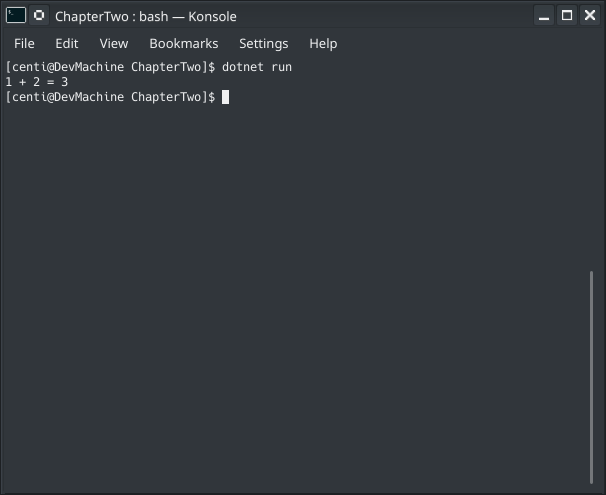
\includegraphics[width=\textwidth]{ChapTwoConsole}
Cela fonctionne comme prévu !
\newpage
\section{Some Backgrounds}
Il se passe peu de choses lorsqu'une fonction avec DllImport est appelée, si c'est la première fois que la fonction est appelée, le Runtime chargera d'abord la bibliothèque externe immédiatement, puis chargera la méthode ''Sum'' lorsque la méthode définie par P/Invoke est appelée, et enfin générera un P/Invoke pour cette fonction pour supporter l'appel à la fonction externe.

Le symbole n'est que cela, un symbole exporté par la bibliothèque C qui peut être résolu à une adresse où se trouve le code ou la variable. Vous pouvez trouver une liste de symboles en exécutant ''objdump -T libChapTwo.so'' sur votre bibliothèque et vous aurez ce qui suit :

\newline \newline
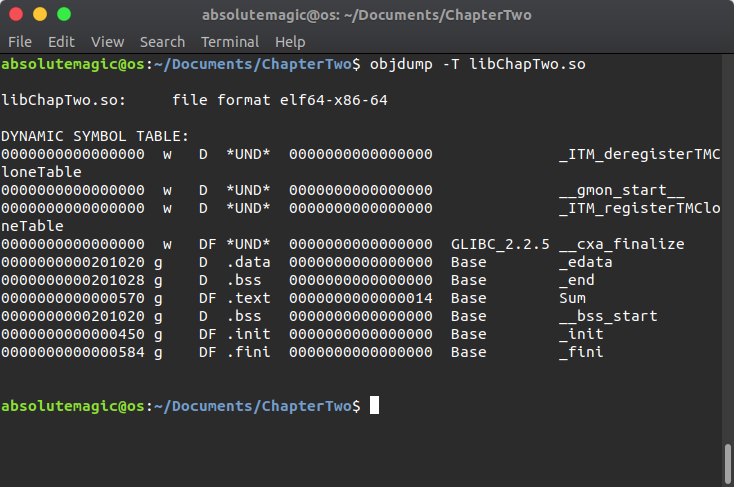
\includegraphics[width=\textwidth]{ChapTwoConsoleTwo}
\newline\newline
Vous remarquerez que le symbole Sum est affiché dans le tableau des symboles de votre bibliothèque, c'est ainsi que la CLR recherche une fonction par nom d'entrée.